\section{Energy and linear momentum}

Physical simulations commonly measure energy. Unexpected fluctuations or drifts 
in the energy often warn us of something askew in our code. Take our bouncing 
rubber ball from the introduction. Its mechanical energy,
\begin{equation*}
  E = \frac{1}{2} m \|\mathbf{v}\|^2 + m|g|y,
\end{equation*}
should remain constant while it flies freely. The absolute value $|g|$ appears 
here instead of plain $g$ because, if you remember, we defined the acceleration 
of gravity as $g = -9.8\ \mathrm{m/s}^2$ in our code. On impact, the ball 
reduced its speed slightly, so we expect a sudden drop in $E$ every time 
the ball hits the floor. As it bounces time and again, leaking more and more 
energy, $E$ will tend towards zero.

Due to numerical rounding in the operations, we shouldn't expect a perfect 
conservation of energy but we obviously want to keep energy fluctuations low, 
below one percent, say. If you have managed to code the algorithm correctly, you 
can usually decrease energy fluctuations by choosing smaller time steps.

Let's verify our predictions about the bouncing ball program by changing the 
output section. We'll set the mass to $100$ grams.
\begin{lstlisting}
%! codeblock: rubberBallEOutput
    if(printEverynSteps > 0
       && step % printEverynSteps == 0) {

      float m = 0.1; /* Mass */

      /* Mechanical energy */
      float E = 0.5*m*(v[0]*v[0] + v[1]*v[1]) - m*g*r[1];

      cout<<step*dt<<" "<<r[0]<<" "<<r[1]<<" "<<E<<endl;
    } //!
%! codeblockend !//
\end{lstlisting}
Note that I wrote \texttt{-m*g*r[1]} instead of \texttt{+m*g*r[1]} due to the 
negative value of \texttt{g}. Figure \ref{rubberBallE} plots the result, which 
agrees with our predictions precisely.

\begin{figure}
  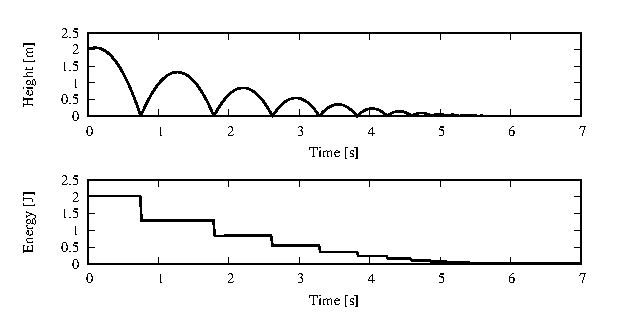
\includegraphics[width = \textwidth]{figures/rubberBallE.eps}
  \caption{\label{rubberBallE}Height (\textit{top}) and mechanical energy 
           (\textit{bottom}) of a one-hundred-gram bouncing ball versus time. 
           The energy remains constant with the ball in free flight, but a 
           fraction is lost when the ball hits the ground.}
\end{figure}

\begin{comment}
rubberBallE.cpp differs only from rubberBall.cpp in the code snippet mentioned 
above.
%! codefile: code/rubberBallE.cpp
# include <iostream>

using std::cout;
using std::endl;

int main(int argc, char * argv[])
{
  /* State of the rubber ball */
  float r[2]; /* Position (measured in metres) */
  float v[2]; /* Velocity (in metres/second) */

  float g = -9.8; /* Acceleration of gravity (in m/s^2) */

  /* Integration parameters */
  int nsteps = 10000; /* Number of time steps to calculate */
  float dt = 0.001; /* Size of time step (in seconds) */
  int printEverynSteps = 20;

  /* Initial conditions */
  r[0] = 0;
  r[1] = 2;
  v[0] = 0.5;
  v[1] = 1;

  /* Euler integration of the equations of motion */
  for(int step = 0; step <= nsteps; ++step) {
    /* New position */
    r[0] = r[0] + v[0]*dt;
    r[1] = r[1] + v[1]*dt;

    /* New velocity */
    v[1] = v[1] + g*dt;

    /* Deal with collisions */
    if(r[1] <= 0 && v[1] < 0) {
      v[0] = 0.9*v[0];
      v[1] = -0.8*v[1];
    }

    /* Output state */
    %! codeinsert: rubberBallEOutput
  }
  cout<<"# Simulated time: "<<nsteps*dt<<" seconds. #"<<endl;
  return 0;
}
%! codeend
\end{comment}

Lennard-Jones energy absent in UAMMD

Shifted potentials

\section{Temperature}

Equipartition theorem. Kinetic temperature.

\section{Thermostats}

Langevin thermostat

Brownian Dynamics

MSD

\section{Structure}

Histograms

RDF

\section{Pressure}

RDF

Virial

Barostats

\section{Check points}

\begin{comment}
List of programs written in this chapter:
%! codeblock: codelist
* `rubberBallE.cpp`: A version of the `rubberBall.cpp` from the introduction 
   which also outputs the mechanical energy of the ball.
%! codeblockend
\end{comment}
